\documentclass[10pt,xcolor=x11names,compress]{beamer}

\usepackage[utf8]{inputenc}
\usepackage[english]{babel}
\usepackage{listings}
\usepackage{tikz}
\usetikzlibrary{arrows.meta,calc,decorations.pathreplacing}
\usepackage{xcolor}
\usepackage{colortbl}
\usetikzlibrary{shadings}

\usepackage{multimedia}
\usepackage{animate}
\usepackage{tikz}
\usetikzlibrary{positioning}
\usepackage{booktabs}

\useoutertheme[subsection=false]{miniframes}
\usecolortheme{seagull}
\usefonttheme[onlymath]{serif}

\setbeamertemplate{blocks}[rounded][shadow=true]
\setbeamercovered{invisible}

\setbeamerfont{mini frame}{series=\bfseries}
\setbeamerfont{section in head/foot}{series=\bfseries}
\setbeamerfont{subsection in head/foot}{series=\bfseries}

\definecolor{colorLeft}{RGB}{16,42,99}
\definecolor{colorRight}{RGB}{214,224,248}
\definecolor{titlefg}{RGB}{255,255,255}
\definecolor{mainColor}{RGB}{16,42,99}

% footline
\setbeamercolor{author in head/foot}{bg=black, fg=white}
\setbeamercolor{title in head/foot}{bg=black, fg=white}
\setbeamercolor{date in head/foot}{bg=black, fg=white}
% navbar
\setbeamercolor{section in head/foot}{bg=black, fg=white}          % section
\setbeamercolor{subsection in head/foot}{bg=black, fg=white}       % subsection
\setbeamercolor{mini frame}{bg=icpcRight, fg=colorLeft}                    % empty miniframe 
\setbeamercolor{mini frame current}{bg=icpcRight, fg=colorLeft}            % current miniframe 

% index
\setbeamercolor{section in toc}{fg=mainColor}
\setbeamercolor{subsection in toc}{fg=black}
\setbeamerfont{section in toc}{series=\bfseries,size=\large}
\setbeamerfont{subsection in toc}{size=\normalsize}

% blocks 
\setbeamercolor{block title}{fg=white, bg=colorLeft}  
\setbeamercolor{block body}{fg=black}   
\setbeamerfont{block title}{series=\normalfont}                 
\setbeamerfont{block body}{series=\normalfont}                 

\setbeamertemplate{section in toc}{%
  \tikz[baseline=(char.base)]{
    \shade[ball color=colorLeft] (0,0) circle (0.2cm); 
    \node[text=white, font=\bfseries\small] (char) at (0,0.1em) {\inserttocsectionnumber}; 
  }%
  \hspace{0.5em}\inserttocsection\par
}

\setbeamertemplate{subsection in toc}{%
  \hspace{2em}%
  \tikz[baseline]{
    \shade[shading=axis, left color=blue, right color=red] (0,0.3em) circle (0.07cm); 
  }%
  \hspace{0.4em}\inserttocsubsection\par
}

% CODE 
\definecolor{mygreen}{rgb}{0,0.6,0}
\definecolor{myblue}{rgb}{0,0,1}
\definecolor{mypink}{rgb}{0.8,0,0.5}
\definecolor{mygray}{rgb}{0.5,0.5,0.5}
\definecolor{lightblue}{rgb}{0.9,0.95,1}

\lstdefinestyle{cppStyle}{
  language=C++,
  % backgroundcolor=\color{lightblue},
  basicstyle=\ttfamily\small,
  keywordstyle=\color{blue}\bfseries,
  commentstyle=\color{mygreen}\itshape,
  stringstyle=\color{myblue},
  numbers=left,
  numberstyle=\tiny\color{mygray},
  stepnumber=1,
  numbersep=8pt,
  showstringspaces=false,
  breaklines=true,
  frame=lines, % Línea arriba y abajo
  rulecolor=\color{cyan},
  tabsize=2
}

\lstset{style=cppStyle}

\newcommand{\highlight}[1]{\textcolor{blue}{\textit{#1}}}




\setbeamertemplate{title page}{
  \begin{center}
    \setbeamercolor{title in titlepage}{%
      use=structure,%
      fg=titlefg,%
      bg=colorLeft!50!colorRight%
    }
    \begin{beamercolorbox}[rounded=true,shadow=true,sep=0.5em,center,wd=0.85\paperwidth]{title in titlepage}
      {\huge\bfseries\inserttitle}
    \end{beamercolorbox}
    \vspace{2em}

    {\large \insertauthor} \\[1em]
    {\normalsize \insertinstitute} \\[1em]
    {\small \insertdate}
    % \begin{figure}[H]
    %   \centering
    %   \includegraphics[width=0.25\linewidth]{logo_cpcfi.png}
    % \end{figure}
  \end{center}
}


\setbeamertemplate{frametitle}{
  \begin{beamercolorbox}[wd=\paperwidth,ht=3.8ex]{frametitle}
    
\begin{tikzpicture}[remember picture,overlay]
      \shade[left color=colorLeft,right color=colorRight] 
      (0,0) rectangle (\paperwidth,4ex);
      \node[anchor=west,text=white,font=\large\bfseries] at (1em,2ex) {\insertframetitle};
    \end{tikzpicture}
  \end{beamercolorbox}
} 

\setbeamertemplate{footline}{%
  \leavevmode
  \hbox to \paperwidth{%
    \begin{beamercolorbox}[wd=.33\paperwidth,ht=4ex,dp=3ex,sep=0pt,left,leftskip=1.5em]{author in head/foot}
      \color{white}\textbf{\insertshortauthor}%
    \end{beamercolorbox}%
    % 
    \begin{beamercolorbox}[wd=.34\paperwidth,ht=4ex,dp=3ex,sep=0pt,center]{title in head/foot}
      \color{white}\textbf{\insertframetitle}
    \end{beamercolorbox}%
    % 
    \begin{beamercolorbox}[wd=.33\paperwidth,ht=4ex,dp=3ex,sep=0pt,right,rightskip=1.5em]{date in head/foot}
      \color{white}\textbf{\insertshortinstitute}%
    \end{beamercolorbox}%
  }%
}

\setbeamercolor{author in head/foot}{bg=black, fg=white}
\setbeamercolor{title in head/foot}{bg=black, fg=white}
\setbeamercolor{date in head/foot}{bg=black, fg=white}


\title[Frame-to-Event Conversion Framework]{Frame-to-Event Conversion Framework}
\author[José Antonio Zarco Romero]{José Antonio Zarco Romero}
\date{\today}
\institute{Technische Hochschule Ingolstadt}

\begin{document}

\begin{frame}
  \titlepage
\end{frame}

\section{Background}

\begin{frame}
  \frametitle{\textbf{Table of Contents}}
  \tableofcontents[
  hideallsubsections=false
  sectionstyle=show/shaded,    
  subsectionstyle=show/shaded/hide, 
  section=1-100                
  ]
\end{frame}

\begin{frame}{Background}

  \begin{columns}[T]


    \column{0.56\textwidth}

    {\Large\bfseries Motivation}

    \vspace{0.1cm}
    \color{colorLeft}\rule{\linewidth}{1pt}

    \vspace{0.1cm}

    \begin{itemize}
    \item Spiking Neural Networks (SNNs) work best with
      \textbf{asynchronous events} instead of RGB frames.

    \item Large RGB datasets are widely available,
      while \textbf{event-camera datasets are limited}.

    \item Goal: reuse existing RGB videos for
      event-based learning.

    \item Enable future models compatible with
      \textbf{both RGB and event cameras}.
    \end{itemize}


    \column{0.44\textwidth}

    \begin{block}{Project Objective}

      Develop a lightweight, classical framework that converts
      RGB video into an event stream

      \vspace{0.4cm}

      \[
        (x,\;y,\;t,\;p)
      \]

      \begin{itemize}
      \item No deep learning
      \item Low computational cost
      \item Validated using DSEC ground truth
      \end{itemize}

    \end{block}

    \vspace{0.4cm}

    \begin{center}
      \Large
      \[
        \boxed{\textbf{RGB Video}\;\rightarrow\;\textbf{Synthetic Events}}
      \]
    \end{center}

  \end{columns}

  % \vfill

  % \begin{block}{Take-away}
  %   SNNs need event data, but RGB dominates available datasets.
  %   This work bridges that gap using a lightweight RGB-to-event conversion framework.
  % \end{block}

\end{frame}

\section{Literature Review}

\begin{frame}
  \frametitle{\textbf{Table of Contents}}
  \tableofcontents[
  hideallsubsections=false
  sectionstyle=show/shaded,    
  subsectionstyle=show/shaded/hide, 
  section=1-100                
  ]
\end{frame}


\begin{frame}{Literature Review}

  \begin{columns}[T]

    \column{0.32\textwidth}

    \begin{block}{ESIM}

      Simulates DVS events using \textbf{3D rendering} and
      \textbf{adaptive sampling} based on optical flow.

      \vspace{0.3cm}

      High physical realism at the expense of
      \textbf{high computational cost}.

    \end{block}

    \column{0.32\textwidth}

    \begin{block}{v2e}

      Converts video into events using
      \textbf{Super-SloMo interpolation}.

      \vspace{0.3cm}

      Includes \textbf{sensor non-idealities} for
      more realistic event generation.

    \end{block}

    \column{0.32\textwidth}

    \begin{block}{Our Approach}

      Inspired by v2e, but designed as a
      \textbf{lightweight classical framework}.

      \vspace{0.3cm}

      Uses temporal intensity differences
      without interpolation or sensor simulation.

    \end{block}

  \end{columns}

\end{frame}

\section{Framework Implementation}

\begin{frame}
  \frametitle{\textbf{Table of Contents}}
  \tableofcontents[
  hideallsubsections=false
  sectionstyle=show/shaded,    
  subsectionstyle=show/shaded/hide, 
  section=1-100                
  ]
\end{frame}


\begin{frame}{Framework Implementation}

  \begin{columns}[T]

    %%%%%%%%%%%%%%%%%%%%%%%%%%%%%%%%%%%%%%%%%%%%%% 
    \column{0.45\textwidth}

    % \begin{block}{Processing Pipeline}
    %   \centering
    %   \vspace{0.2cm}
    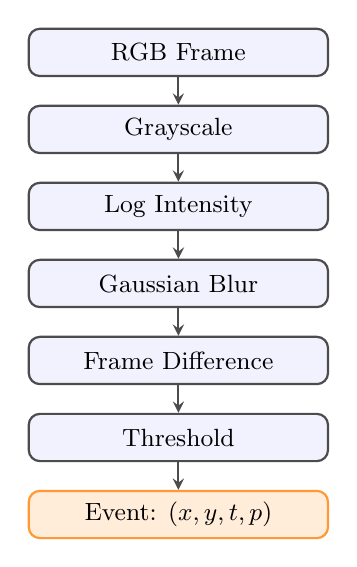
\begin{tikzpicture}[
      node distance=0.35cm,
      box/.style={draw=black!70, fill=blue!5, thick, rounded corners, align=center, font=\small, minimum width=3.8cm, minimum height=0.6cm},
      arrow/.style={thick, ->, >=stealth, draw=black!70}
      ]
      
      % Nodes
      \node (rgb) [box] {RGB Frame};
      \node (gray) [box, below=of rgb] {Grayscale};
      \node (log) [box, below=of gray] {Log Intensity};
      \node (blur) [box, below=of log] {Gaussian Blur};
      \node (diff) [box, below=of blur] {Frame Difference};
      \node (thresh) [box, below=of diff] {Threshold};
      \node (event) [box, fill=orange!15, draw=orange!80, below=of thresh] {Event: $(x, y, t, p)$};
      
      % Arrows
      \draw [arrow] (rgb) -- (gray);
      \draw [arrow] (gray) -- (log);
      \draw [arrow] (log) -- (blur);
      \draw [arrow] (blur) -- (diff);
      \draw [arrow] (diff) -- (thresh);
      \draw [arrow] (thresh) -- (event);
      
    \end{tikzpicture}
    % \vspace{0.2cm}
    % \end{block}

    %%%%%%%%%%%%%%%%%%%%%%%%%%%%%%%%%%%%%%%%%%%%%% 
    \column{0.5\textwidth}

    \begin{block}{Event Generation}
      For every pixel, calculate the intensity change:
      \[
        \Delta L = L_t - L_{t-1}
      \]
      Generate an event if the change exceeds $\theta$:
      \[
        p = 
        \begin{cases} 
          +1, & \text{if } \Delta L > \theta \\ 
          -1, & \text{if } \Delta L < -\theta 
        \end{cases}
      \]
    \end{block}

    % \vspace{0.2cm}

    % \begin{block}{Command-Line Interface}
    \scriptsize
    \texttt{\textbf{\$} uv run python -m framework.cli \textbackslash} \\
    \texttt{\hspace*{0.5cm}-i input.mp4 -o results \textbackslash} \\
    \texttt{\hspace*{0.5cm}-t 0.1 --resize 640 480 --video}
    % \end{block}

  \end{columns}

\end{frame}

\section{Evaluation}

\subsection{Visual Comparison}

\begin{frame}
  \frametitle{\textbf{Table of Contents}}
  \tableofcontents[
  hideallsubsections=false
  sectionstyle=show/shaded,    
  subsectionstyle=show/shaded/hide, 
  section=1-100                
  ]
\end{frame}

\begin{frame}{Visual Comparison}

  \small
  Evaluation on \textbf{Zurich City 13 a} sequence (50 ms temporal windows).

  \vspace{0.4cm}

  \begin{columns}[T]

    \column{0.49\textwidth}

    \begin{block}{Original DSEC Event Camera}

      \begin{center}

        \movie[
        width=\linewidth,
        height=0.5\textheight,
        showcontrols,
        autostart,
        loop
        ]
        {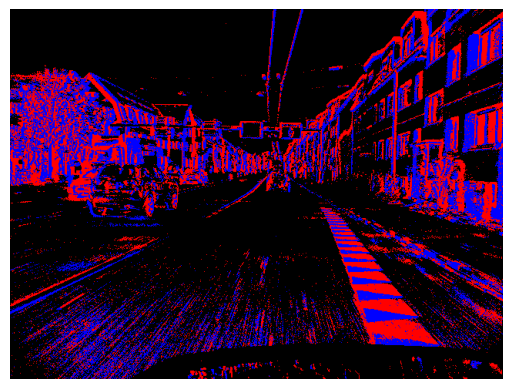
\includegraphics[width=\linewidth]{figures/dsec_preview.png}}
        {figures/dsec.mp4}

      \end{center}

    \end{block}

    \column{0.49\textwidth}

    \begin{block}{Generated Synthetic Events}

      \begin{center}

        \movie[
        width=\linewidth,
        height=0.5\textheight,
        showcontrols,
        autostart,
        loop
        ]
        {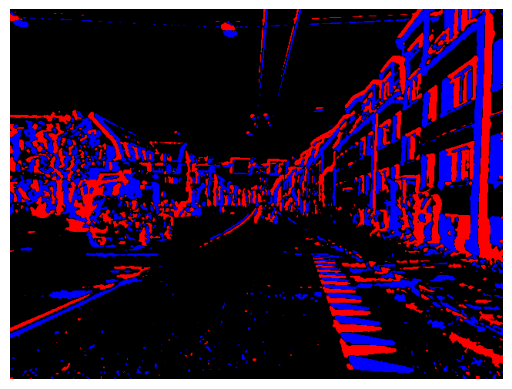
\includegraphics[width=\linewidth]{figures/framework_preview.png}}
        {figures/framework.mp4}

      \end{center}

    \end{block}

  \end{columns}

\end{frame}

\subsection{Quantitative Results}

\begin{frame}
  \frametitle{\textbf{Table of Contents}}
  \tableofcontents[
  hideallsubsections=false
  sectionstyle=show/shaded,    
  subsectionstyle=show/shaded/hide, 
  section=1-100                
  ]
\end{frame}

\begin{frame}{Quantitative Results}

  \begin{columns}[T]

    \column{0.60\textwidth}

    %\begin{block}{Event Count Correlation}

      \begin{center}
        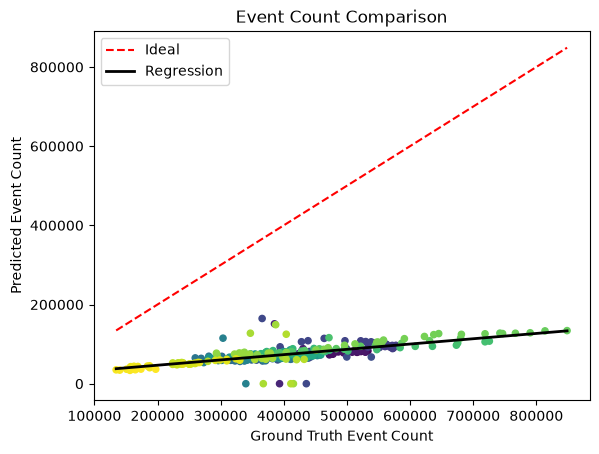
\includegraphics[
        width=\linewidth,
        height=0.6\textheight,
        keepaspectratio
        ]{figures/linear_regression.png}
      \end{center}
      \begin{center}
        \small
        Pearson Correlation:
        \textbf{0.709} \\ Tracks scene activity accurately.
      \end{center}

    %\end{block}
    \column{0.37\textwidth}

    \begin{block}{Sparsity Yield}

      \vspace{0.3cm}

      \begin{center}

        {\fontsize{20}{20}\selectfont
          \textcolor{blue}{\textbf{18.3\%}}}

      \end{center}

      % \vspace{0.1cm}

      \centering
      \small
      Events retained with respect to
      ground-truth events.

      % \vspace{0.15cm}

      % Noise is reduced while preserving
      % scene dynamics.

    \end{block}

    \vspace{0.1cm}

    \begin{block}{Spatial Precision}

      \vspace{0.2cm}

      \begin{center}

        {\fontsize{20}{20}\selectfont
          \textcolor{blue}{\textbf{93.5\%}}}

      \end{center}

      % \vspace{0.1cm}

      \centering
      \small
      Spatial F1-score \textbf{0.86}

      Events happen in the correct regions.

    \end{block}

  \end{columns}

\end{frame}

\subsection{Comparison with v2e}

\begin{frame}
  \frametitle{\textbf{Table of Contents}}
  \tableofcontents[
  hideallsubsections=false
  sectionstyle=show/shaded,    
  subsectionstyle=show/shaded/hide, 
  section=1-100                
  ]
\end{frame}

\begin{frame}{Comparison with v2e}

\centering
\small

\renewcommand{\arraystretch}{1.2}

\begin{tabular}{lcc}
\rowcolor{colorLeft}
\color{white}\textbf{Metric} &
\color{white}\textbf{v2e} &
\color{white}\textbf{Proposed Framework} \\
\hline
Event Count         & 75.8 M          & 27.9 M \\
DSEC Percentage     & 49.79\%         & 18.29\% \\
Pearson Correlation & \textbf{0.867}  & 0.709 \\
Precision (ALL)     & 0.9127          & \textbf{0.9356} \\
Recall (ALL)        & \textbf{0.9494} & 0.8093 \\
F1-score (ALL)      & \textbf{0.9291} & 0.8675 \\
\end{tabular}

\vspace{0.45cm}
\end{frame}

\subsection{Object Detection}

\begin{frame}
  \frametitle{\textbf{Table of Contents}}
  \tableofcontents[
  hideallsubsections=false
  sectionstyle=show/shaded,    
  subsectionstyle=show/shaded/hide, 
  section=1-100                
  ]
\end{frame}


\begin{frame}{Object Detection}
  \begin{figure}[h]
        \centering
        
\includegraphics[width=0.75\linewidth]{figures/twl_spike_yolo.png}
      \end{figure}
  \footnotesize
  Tested with pre-trained \textbf{TWL SpikeYOLO}
  % (zero-shot transfer).           

  % \vspace{0.4cm}

  % \begin{columns}[T]

  %   \column{0.49\textwidth}

  %   \begin{block}{DSEC Events}

  %     \begin{figure}[h]
  %       \centering
  %       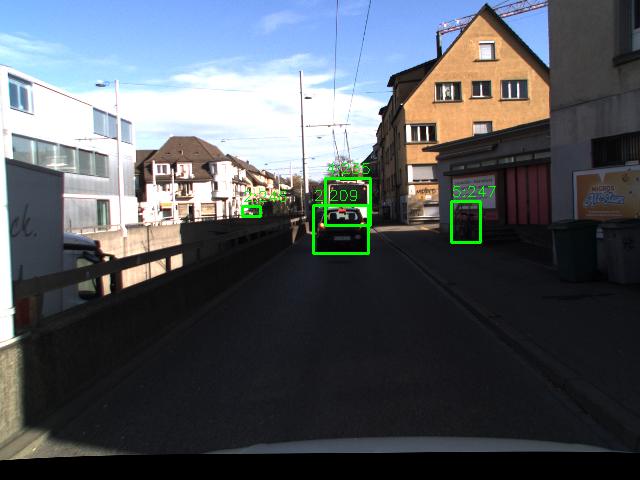
\includegraphics[width=\linewidth]{figures/object_detection/dsec/gt.png}
  %     \end{figure}

  %   \end{block}

  %   \column{0.49\textwidth}

  %   \begin{block}{Synthetic Events}

  %     \begin{figure}[h]
  %       \centering
  %       
\includegraphics[width=\linewidth]{figures/object_detection/framework/img/frame_001.png}
  %     \end{figure}

  %   \end{block}


  % \end{columns}

  % \vspace{0.3cm}

  % The detector successfully identifies several vehicles and pedestrians when using the original DSEC event stream. In contrast, when using the generated events, only a small number of detections remain.
  % \begin{alertblock}{Insight}
  %   \textbf{Insight:}
  %   While structurally similar, the statistical distribution differs significantly. Networks trained purely on real sensors cannot generalize to synthetic data without domain adaptation or fine-tuning.
  % \end{alertblock}

\end{frame}

\section{Conclusions}

\begin{frame}{Conclusions}

  \begin{columns}[T]

    \column{0.52\textwidth}

    {\Large\bfseries Achievements}

    \vspace{0.1cm}
    \color{colorLeft}\rule{\linewidth}{1pt}

    \vspace{0.1cm}

    \begin{itemize}
    \item[$\checkmark$] Lightweight: Avoids expensive rendering \& sub-frame interpolation
    \item[$\checkmark$] Preserves scene dynamics and spatial event locations.
    \item[$\checkmark$] Strong correlation with real event activity
      ($r=0.709$).
    \item[$\checkmark$] Reduces redundant events while maintaining moving structures.
    \end{itemize}

    \column{0.48\textwidth}

    % {\Large\bfseries Limitations}

    % \vspace{0.1cm}
    % \color{colorRight}\rule{\linewidth}{1pt}

    % \vspace{0.1cm}

    % \begin{itemize}
    % \item[$\rightarrow$] Event statistics differ from real DVS cameras.

    % \item[$\rightarrow$] Zero-shot object detection does not generalize.

    % \item[$\rightarrow$] Domain adaptation or fine-tuning is required for SNNs.
    % \end{itemize}

  \end{columns}

  \vfill

  \begin{center}
    \Large\bfseries
    Thank you!
  \end{center}

  \begin{center}
    \small
    \texttt{github.com/jzarcoo/Frame-to-Event-Conversion-Framework}
  \end{center}

\end{frame}



\begin{frame}{Bibliography}
  \begin{thebibliography}{9}

  \bibitem{dsec} Gehrig, M., Aarents, W., Gehrig, D., & Scaramuzza, D. (2021). DSEC: A stereo event camera dataset for driving scenarios. IEEE Robotics and Automation Letters. \url{https://doi.org/10.1109/LRA.2021.3068942}
    
  \bibitem{esim} Gehrig, D., Rebecq, H., \& Scaramuzza, D. (2018). \textit{ESIM: an Open Event Camera Simulator}. Robotics and Perception Group, Depts. Informatics and Neuroinformatics, University of Zurich and ETH Zurich. \url{https://rpg.ifi.uzh.ch/docs/CORL18_Rebecq.pdf}

  \bibitem{dsec-det} Gehrig, D., & Scaramuzza, D. (2024). Low latency automotive vision with event cameras. Nature.

  \end{thebibliography}
  
\end{frame}
\begin{frame}{Bibliography}
  \begin{thebibliography}{9}
    
  \bibitem{model} Khitushkin, K.S., Isakov, T.T., Bakhshiev, A.V. (2026). Using Spiking Neural Networks for Event and Multimodal Data Processing in Object Detection Tasks. In: Kryzhanovsky, B., Dunin-Barkowski, W., Redko, V., Tiumentsev, Y., Klimov, V.V. (eds) Advances in Neural Computation, Machine Learning, and Cognitive Research IX. NEUROINFORMATICS 2025. Studies in Computational Intelligence, vol 1241. Springer, Cham. \url{https://doi.org/10.1007/978-3-032-07690-8_10}

  \bibitem{v2e} Y. Hu, S-C. Liu, and T. Delbruck. v2e: From Video Frames to Realistic DVS Events. In 2021 IEEE/CVF Conference on Computer Vision and Pattern Recognition Workshops (CVPRW), URL: https://arxiv.org/abs/2006.07722, 2021
    
  \end{thebibliography}
  
\end{frame}


\end{document}

